\subsection{Caso d'uso UC8: Gestione delle domande}
	\label{UC8}
	\begin{figure}[h]
		\centering
			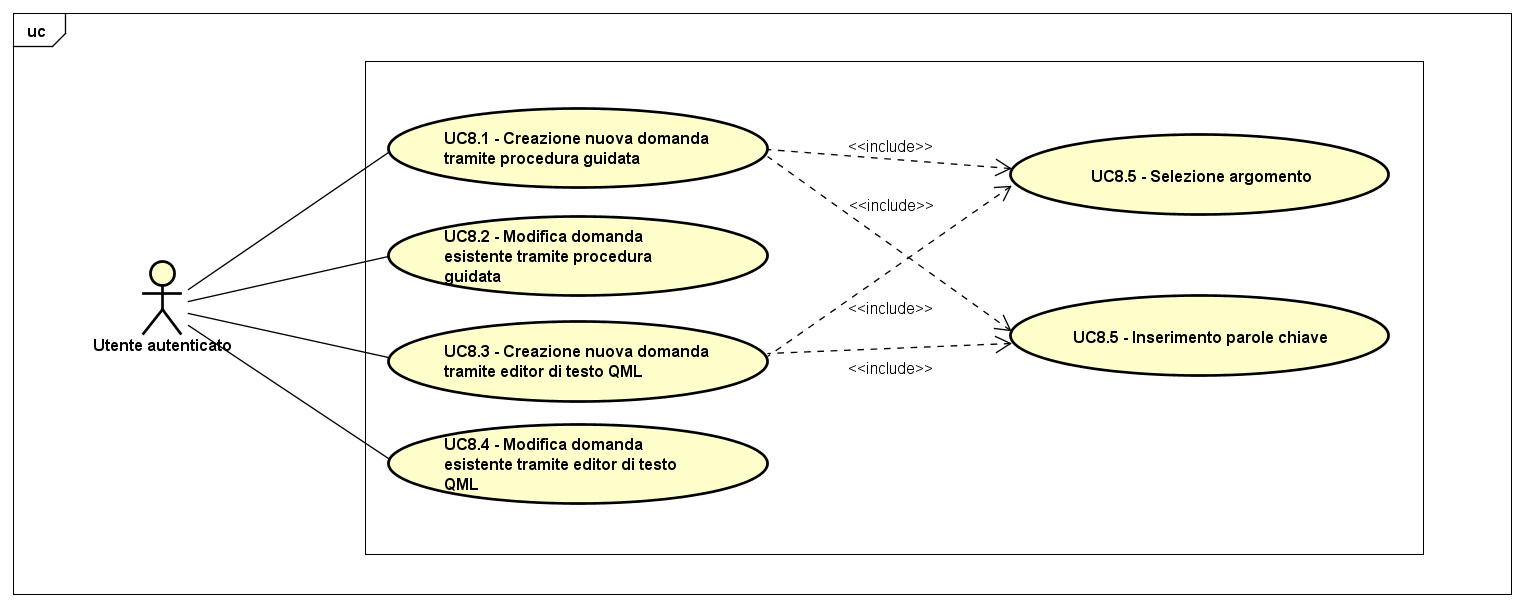
\includegraphics[scale=0.45,keepaspectratio]{UML/UC8.png}
		\caption{UC8: Gestione delle domande}
	\end{figure}
	\FloatBarrier
	\begin{itemize}
		\item
			\textbf{Attori}: utente autenticato, utente autenticato pro;
		\item		
			\textbf{Descrizione}: lo scopo di questa funzionalità è offrire agli attori la possibilità di creare e modificare domande;
		\item
			\textbf{Precondizione}: gli attori sono autenticati presso il sistema; 
		\item
			\textbf{Postcondizione}: gli attori hanno compiuto una delle operazioni appartenenti a questa funzionalità;
		\item
			\textbf{Scenario principale}:
	       		\begin{enumerate}
					\item
					Gli attori creano una nuova domanda [UC8.1];
					\item
					Gli attori modificano una domanda [UC8.2].
	 			\end{enumerate}
	\end{itemize}
\subsubsection{Caso d'uso UC8.1: Creazione nuova domanda}
	\label{UC8.1}
	\begin{figure}[h]
		\centering
			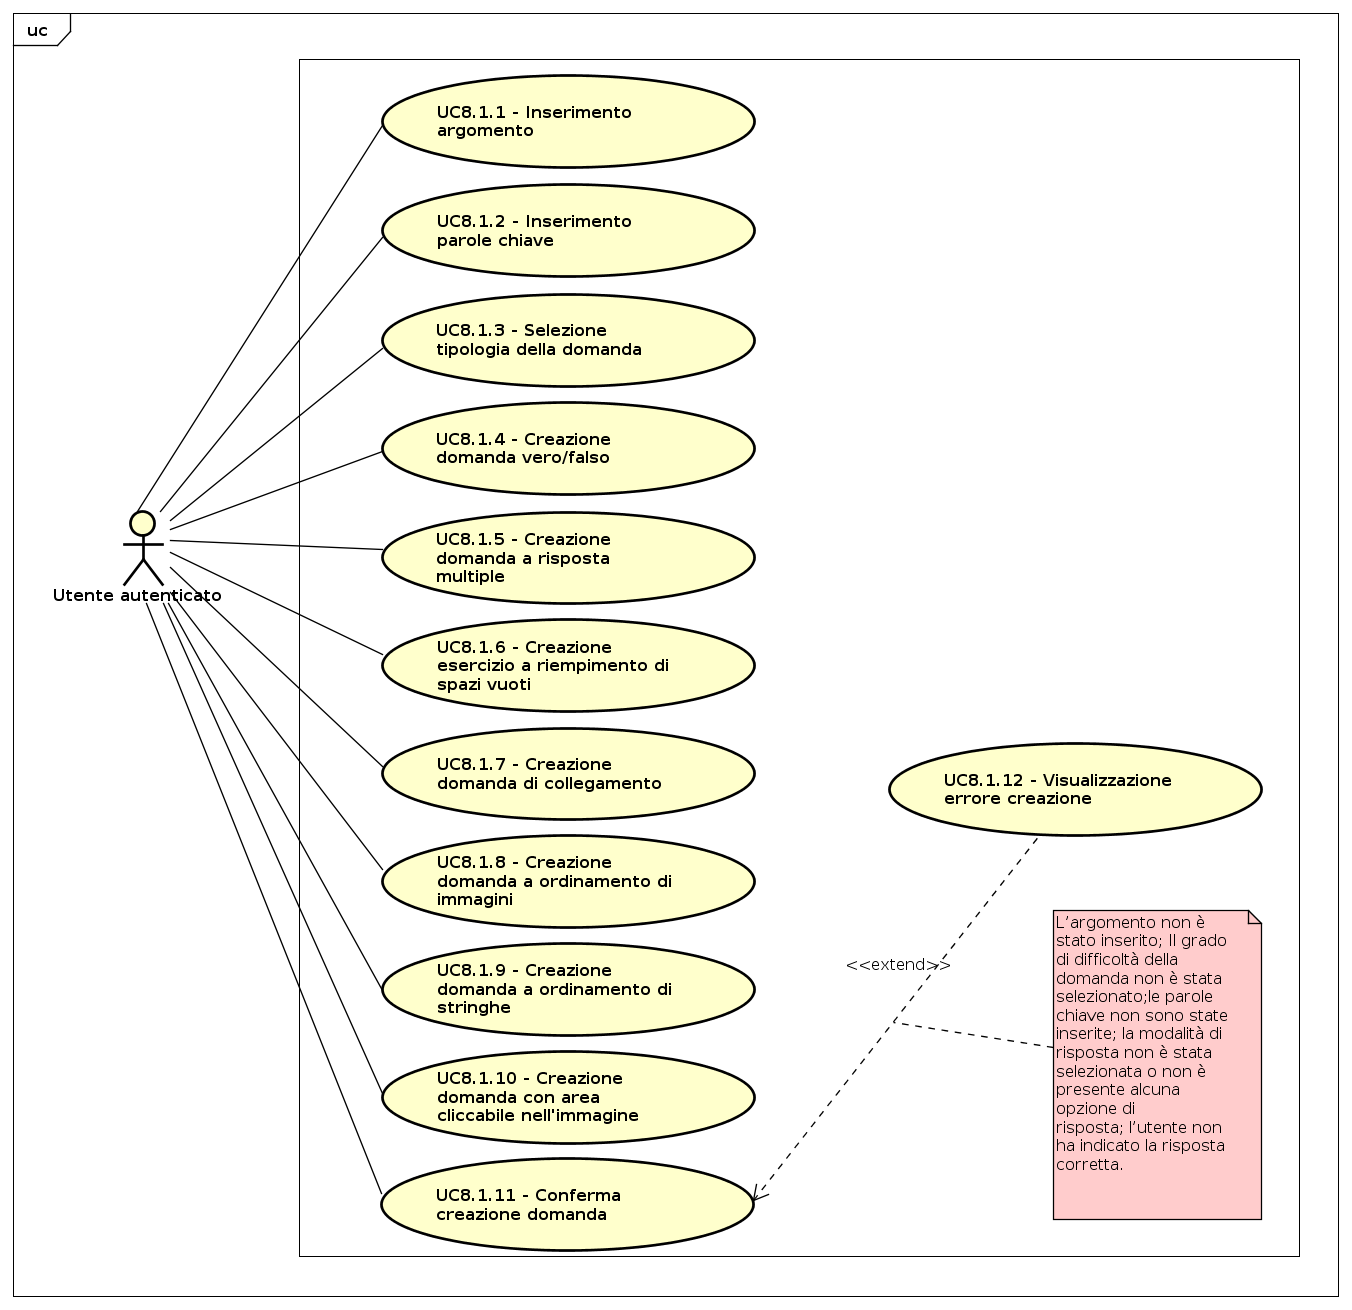
\includegraphics[scale=0.45,keepaspectratio]{UML/UC8_1.png}
		\caption{UC8.1: Creazione nuova domanda}
	\end{figure}
	\FloatBarrier
	\begin{itemize}
		\item
			\textbf{Attori}: utente autenticato, utente autenticato pro;
		\item		
			\textbf{Scopo e descrizione}: gli attori possono creare una nuova domanda, utile all'apprendimento di un determinato argomento;
		\item
			\textbf{Precondizione}: gli attori hanno selezionato l'opzione per la creazione della domanda;
		\item
			\textbf{	Postcondizione}: gli attori ricevono conferma dell'avvenuta creazione;		
		\item
			\textbf{Scenario principale}:
	       		\begin{enumerate}
					\item
					L'utente inserisce l'argomento relativo alla nuova domanda[UC8.1.1];
					\item
					L'utente inserisce le parole chiave relative alla nuova domanda [UC8.1.2];
					\item
					L'utente inserisce il testo della domanda [UC8.1.3];
					\item
					L'utente deve selezionare la modalità di risposta ed eventualmente inserire le opzioni di risposta [UC8.1.4];
					\item
					L'utente deve indicare la risposta corretta [UC8.1.5];
					\item
					L'utente conferma la creazione della domanda [UC8.1.6].
	 			\end{enumerate}
	 	\item
			\textbf{Estensione}: L'utente visualizza un messaggio d'errore di conferma [UC8.1.8];
	 	\item
	 		\textbf{Scenario alternativo}: possono verificarsi uno o più di questi scenari:
				\begin{itemize}
					\item[-] 	
						L'argomento non è stato inserito;
					\item[-] 
						Le parole chiave non sono state inserite;
					\item[-] 
						La modalità di risposta non è stata selezionata o non è presente alcuna opzione di risposta; 
					\item[-]
						La risposta corretta non è stata indicata.	
				\end{itemize}
			In tal caso il sistema ripresenta il modulo di creazione della domanda, presentando un messaggio d'errore.
	\end{itemize}
	\subsubsection{Caso d'uso UC8.1.1: Selezione argomento}
	\begin{itemize}
		\item
			\textbf{Attori}: utente autenticato, utente autenticato pro;
		\item
			\textbf{Scopo e descrizione}: gli attori, tramite uno strumento di selezione offerto dal sistema, possono indicare un argomento tra quelli presenti;
		\item		
			\textbf{Precondizione}: il sistema presenta all'utente autenticato uno strumento di selezione per assegnare alla nuova domanda un argomento;
		\item
			\textbf{Postcondizione}: l'argomento è stato selezionato.
		\item
			\textbf{Scenario principale}:
				\begin{enumerate}
					\item 	
						Gli attori selezionano l'argomento da assegnare alla nuova domanda	
				\end{enumerate}
	\end{itemize}	
	\subsubsection{Caso d'uso UC8.1.2: Inserimento parole chiave}
	\begin{itemize}
		\item
			\textbf{Attori}: utente autenticato, utente autenticato pro;
		\item
			\textbf{Scopo e descrizione}: gli attori possono inserire le parole chiave relative alla nuova domanda per facilitare la ricerca di una domanda;
		\item		
			\textbf{Precondizione}: il sistema presenta all'utente autenticato il campo dati per l'inserimento delle parole chiave;
		\item
			\textbf{Postcondizione}: l'inserimento delle parole chiave è avvenuto.
		\item
			\textbf{Scenario principale}:
				\begin{enumerate}
					\item 	
						Gli attori inseriscono le parole chiave relative alla nuova domanda	
				\end{enumerate}
	\end{itemize}
	\subsubsection{Caso d'uso UC8.1.3: Inserimento testo della domanda}
	\begin{itemize}
		\item
			\textbf{Attori}: utente autenticato, utente autenticato pro;
		\item
			\textbf{Scopo e descrizione}: gli attori inseriscono il testo della domanda;
		\item		
			\textbf{Precondizione}: il sistema presenta all'utente autenticato il campo dati per l'inserimento del testo della domanda;
		\item
			\textbf{Postcondizione}: l'inserimento del testo della domanda è avvenuto.
	\end{itemize}
	\subsubsection{Caso d'uso UC8.1.4: Selezione modalità di risposta}
	\label{UC8.1.5}
	\begin{figure}[h]
		\centering
			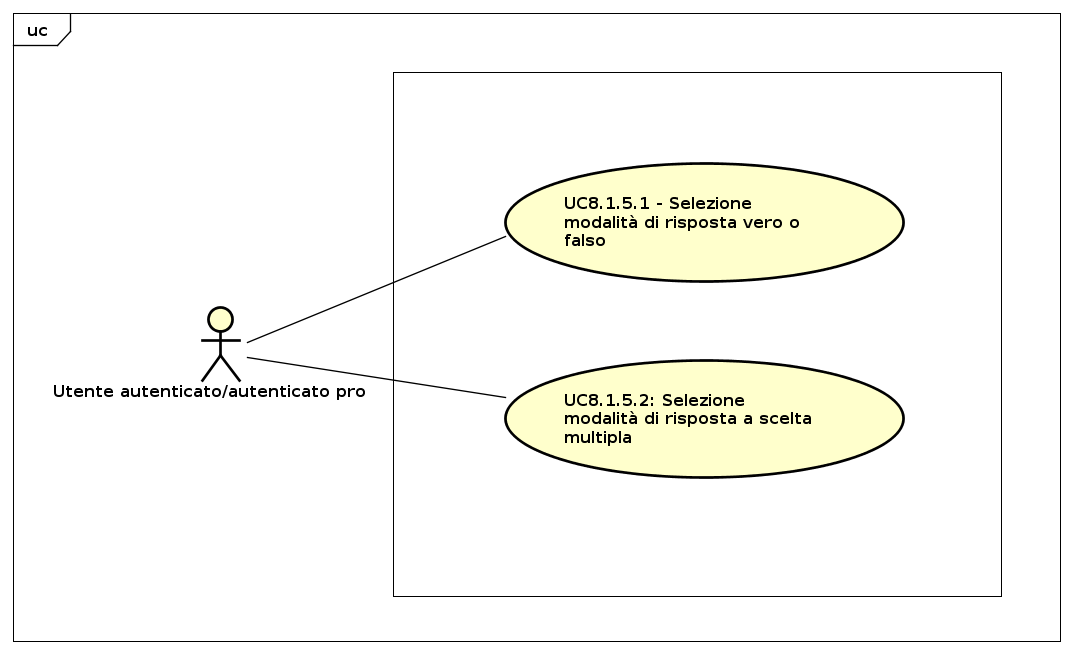
\includegraphics[scale=0.5,keepaspectratio]{UML/UC8_1_5.png}
		\caption{UC8.1.5: Selezione modalità di risposta}
	\end{figure}
	\FloatBarrier
	\begin{itemize}
		\item
			\textbf{Attori}: utente autenticato, utente autenticato pro;
		\item
			\textbf{Scopo e descrizione}: l'utente autenticato seleziona la modalità di risposta preferita;
		\item		
			\textbf{Precondizione}: il sistema presenta all'utente autenticato le checkbox per selezionare la modalità di risposta preferita;
		\item
			\textbf{Scenario principale}:
	       		\begin{enumerate}
					\item
					L'utente seleziona la modalità di risposta vero o falso [UC8.1.5.1];
					\item
					L'utente seleziona la modalità di risposta a scelta multipla [UC8.1.5.2]	       		
	       		\end{enumerate}
		\item
			\textbf{Postcondizione}: Una modalità di risposta è stata selezionata.
	\end{itemize}
	\subsubsection{Caso d'uso UC8.1.4.1: Selezione modalità di risposta vero o falso}
	\begin{itemize}
		\item
			\textbf{Attori}: Utente autenticato, utente autenticato pro;
		\item
			\textbf{Scopo e descrizione}: l'utente autenticato seleziona la modalità di risposta vero o falso;
		\item		
			\textbf{Precondizione}: il sistema presenta all'utente autenticato la checkbox per selezionare la modalità di risposta vero o falso;
		\item
			\textbf{Postcondizione}: la modalità di risposta vero o falso è stata selezionata.
	\end{itemize}
	\subsubsection{Caso d'uso UC8.1.4.2: Selezione modalità di risposta a scelta multipla}
	\label{UC8.1.5.2}
	\begin{figure}[h]
		\centering
			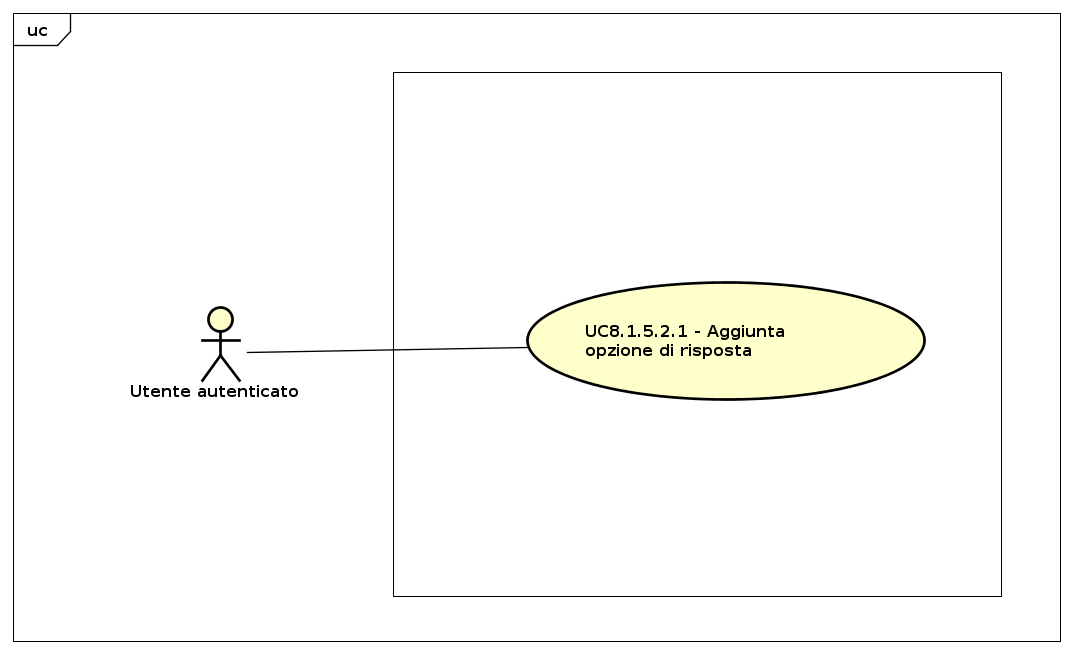
\includegraphics[scale=0.5,keepaspectratio]{UML/UC8_1_5_2.png}
		\caption{UC8.1.5.2: Selezione modalità di risposta a scelta multipla}
	\end{figure}
	\FloatBarrier	
	\begin{itemize}
		\item
			\textbf{Attori}: Utente autenticato, utente autenticato pro;
		\item
			\textbf{Scopo e descrizione}: L'utente autenticato seleziona la modalità di risposta a scelta multipla;
		\item		
			\textbf{Precondizione}: Il sistema presenta all'utente autenticato la checkbox per selezionare la modalità di risposta a scelta multipla;
		\item
			\textbf{Scenario principale}:
				\begin{enumerate}
					\item 	
						L'utente aggiunge due o più opzioni di risposta [UC8.1.5.2.1];	
				\end{enumerate}
		\item
			\textbf{Postcondizione}: La modalità di risposta a scelta multipla è stata selezionata.
	\end{itemize}
	\subsubsection{Caso d'uso UC8.1.4.2.1: Aggiunta opzione di risposta}
		\begin{itemize}
		\item
			\textbf{Attori}: Utente autenticato, utente autenticato pro;
		\item
			\textbf{Scopo e descrizione}: L'utente autenticato aggiunge due o più opzioni di risposta;
		\item		
			\textbf{Precondizione}: Il sistema presenta all'utente autenticato lo spazio per aggiungere una opzione di risposta;
		\item		
			\textbf{Postcondizione}: L'utente autenticato ha aggiunto le opzioni di  risposta;
		\end{itemize}
	\subsubsection{Caso d'uso UC8.1.5: Indicazione risposta corretta}
		\begin{itemize}
		\item
			\textbf{Attori}: Utente autenticato, utente autenticato pro;
		\item
			\textbf{Scopo e descrizione}: gli attori indicano la risposta corretta;
		\item		
			\textbf{Precondizione}: gli attori hanno selezionato la modalità di risposta ed inserito le eventuali opzioni nel caso avesse scelto la modalità a scelta multipla. Il sistema predispone un strumento di selezione per indicare la risposta corretta.
		\item		
			\textbf{Postcondizione}: gli attori hanno indicato la risposta corretta.
		\end{itemize}
	\subsubsection{Caso d'uso UC8.1.6: Conferma creazione}
	\begin{itemize}
		\item
			\textbf{Attori}: utente autenticato, utente autenticato pro;
		\item
			\textbf{Scopo e descrizione}: gli attori possono confermare la creazione della domanda;
		\item		
			\textbf{Precondizione}: il sistema presenta all'utente autenticato l'opzione per compiere questa operazione;
		\item
			\textbf{Postcondizione}: il sistema ha ricevuto i dati per la creazione;
		\item
			\textbf{Scenario Principale}:  
					\begin{enumerate}
						\item
							Gli attori confermano la creazione della domanda.
					\end{enumerate}
	\end{itemize}	
	\subsubsection{Caso d'uso UC8.1.7: Visualizzazione errore creazione}
	\begin{itemize}
		\item
			\textbf{Attori}: utente autenticato, utente autenticato pro;
		\item
			\textbf{Scopo e descrizione}: gli attori possono visualizzare un messaggio d'errore nel caso si fossero verificati uno o più scenari alternativi;
		\item		
			\textbf{Precondizione}: il sistema ha ricevuto dei dati errati per la creazione della domanda;
		\item
			\textbf{Postcondizione}: il sistema mostra un messaggio d'errore;
	\end{itemize}	
	\subsubsection{Caso d'uso UC8.2: Modifica domanda esistente}
	\label{UC8.2}
	\begin{figure}[h]
		\centering
			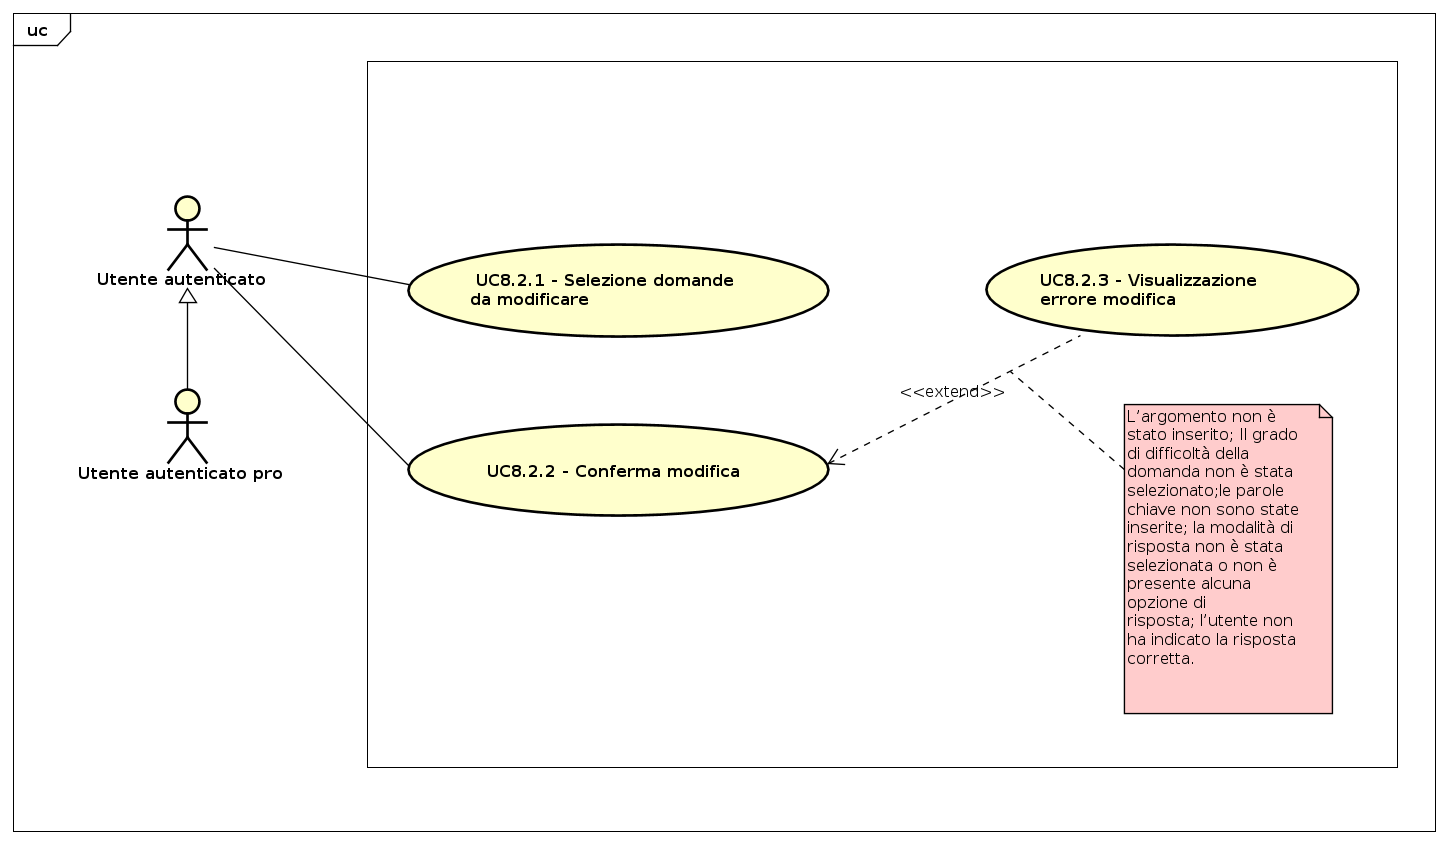
\includegraphics[scale=0.45,keepaspectratio]{UML/UC8_2.png}
		\caption{UC8.2: Modifica domanda esistente}
	\end{figure}
	\FloatBarrier
	\begin{itemize}
		\item
			\textbf{Attori}: utente autenticato, utente autenticato pro;
		\item		
			\textbf{Scopo e descrizione}: L'utente autenticato modifica una domanda da lui in precedenza creata per correggere errori ortografici o sintattici;
		\item
			\textbf{Precondizione}: L'utente autenticato ha selezionato l'opzione per modificare una domanda;
		\item
			\textbf{	Postcondizione}: L'utente riceve conferma dell'avvenuta modifica.
		\item
			\textbf{Scenario principale}:
	       		\begin{enumerate}
					\item
					L'utente modifica l'argomento relativo alla domanda selezionata[UC8.2.1];
					\item
					L'utente modifica il grado di difficoltà relativo alla domanda selezionata [UC8.2.2];
					\item
					L'utente modifica le parole chiave relative alla domanda selezionata [UC8.2.3];
					\item
					L'utente modifica il testo relativo alla domanda selezionata [UC8.2.4];
					\item
					L'utente modifica la modalità di risposta ed eventualmente modifica le opzioni di risposta [UC8.2.5];
					\item
					L'utente modifica la risposta corretta [UC8.2.6];
					\item
					L'utente conferma la modifica della domanda [UC8.2.7].
	 			\end{enumerate}
	 	\item
			\textbf{Estensione}: L'utente visualizza un messaggio d'errore di conferma [UC8.2.8].
	 	\item
	 		\textbf{Scenario alternativo}: possono verificarsi uno o più di questi scenari:
				\begin{itemize}
					\item[-] 	
						L'argomento non è stato inserito;
					\item[-] 
    						Il grado di difficoltà della domanda non è stata selezionato;
					\item[-] 
						Le parole chiave non sono state inserite;
					\item[-] 
						La modalità di risposta non è stata selezionata o non è presente alcuna opzione di risposta; 
					\item[-]
						L'utente non ha indicato la risposta corretta.	
				\end{itemize}
			In tal caso il sistema ripresenta il modulo di modifica della domanda, presentando un messaggio d'errore.
	\end{itemize}
	\subsubsection{Caso d'uso UC8.2.1: Modifica argomento}
	\begin{itemize}
		\item
			\textbf{Attori}: utente autenticato, utente autenticato pro;
		\item
			\textbf{Scopo e descrizione}: l'utente autenticato modifica il campo dati argomento;
		\item		
			\textbf{Precondizione}: il sistema presenta all'utente autenticato il campo dati per modificare l'argomento;
		\item
			\textbf{Postcondizione}: il campo dato argomento è stato modificato.
	\end{itemize}	
	\subsubsection{Caso d'uso UC8.2.2: Modifica grado di difficoltà della domanda}
	\begin{itemize}
		\item
			\textbf{Attori}: utente autenticato, utente autenticato pro;
		\item
			\textbf{Scopo e descrizione}: l'utente autenticato modifica il grado di difficoltà della domanda;
		\item		
			\textbf{Precondizione}: il sistema presenta all'utente autenticato lo spazio per modificare il grado di difficoltà della domanda;
		\item
			\textbf{Postcondizione}: il grado di difficoltà della domanda è stato modificato.
	\end{itemize}	
	\subsubsection{Caso d'uso UC8.2.3: Modifica parole chiave}
	\begin{itemize}
		\item
			\textbf{Attori}: utente autenticato, utente autenticato pro;
		\item
			\textbf{Scopo e descrizione}: l'utente autenticato modifica le parole chiave relative alla domanda selezionata;
		\item		
			\textbf{Precondizione}: il sistema presenta all'utente autenticato il campo dati per l'inserimento delle parole chiave;
		\item
			\textbf{Postcondizione}: l'inserimento delle parole chiave è avvenuto.
	\end{itemize}
	\subsubsection{Caso d'uso UC8.2.4: Modifica testo della domanda}
	\begin{itemize}
		\item
			\textbf{Attori}: utente autenticato, utente autenticato pro;
		\item
			\textbf{Scopo e descrizione}: l'utente autenticato modifica il testo della domanda;
		\item		
			\textbf{Precondizione}: il sistema presenta all'utente autenticato il campo dati per la modifica del testo della domanda;
		\item
			\textbf{Postcondizione}: la modifica del testo della domanda è avvenuto.
	\end{itemize}
	\subsubsection{Caso d'uso UC8.2.5: Modifica modalità di risposta}
	\label{UC8.2.5}
	\begin{figure}[h]
		\centering
			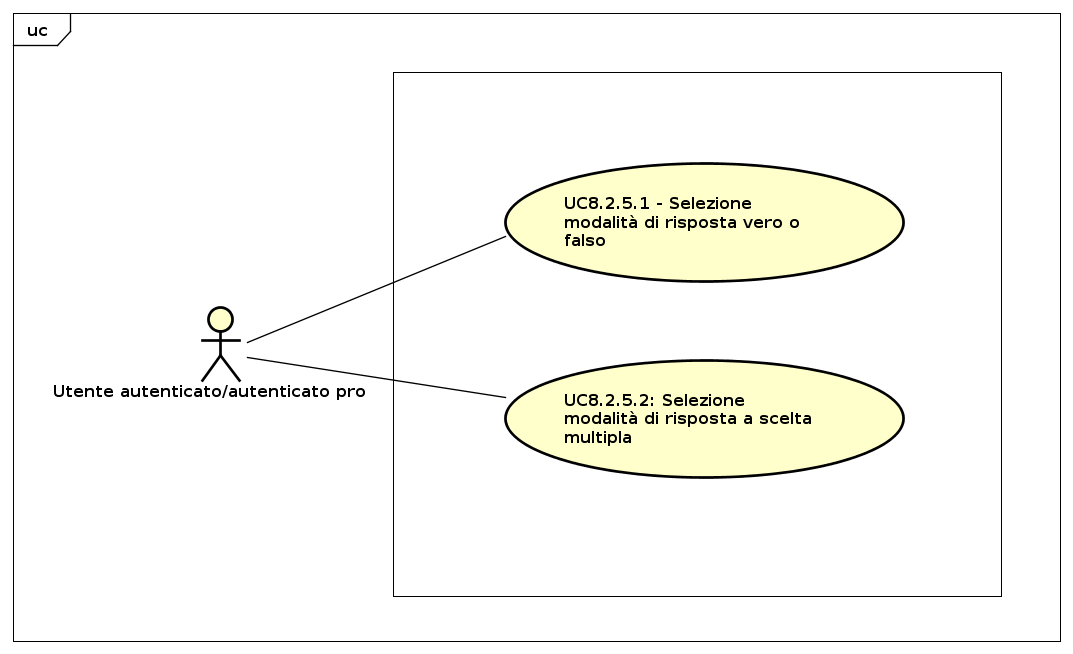
\includegraphics[scale=0.45,keepaspectratio]{UML/UC8_2_5.png}
		\caption{UC8.2.5: Modifica modalità di risposta}
	\end{figure}
	\FloatBarrier
	\begin{itemize}
		\item
			\textbf{Attori}: utente autenticato, utente autenticato pro;
		\item
			\textbf{Scopo e descrizione}: l'utente autenticato modifica la modalità di risposta preferita;
		\item		
			\textbf{Precondizione}: il sistema presenta all'utente autenticato le checkbox per modificare la modalità di risposta;
		\item
			\textbf{Scenario principale}:
	       		\begin{enumerate}
					\item
					L'utente seleziona la modalità di risposta vero o falso [UC8.2.5.1];
					\item
					L'utente seleziona la modalità di risposta a scelta multipla [UC8.2.5.2].
	       		\end{enumerate}
		\item
			\textbf{Postcondizione}: Una modalità di risposta è stata selezionata.
	\end{itemize}
	\subsubsection{Caso d'uso UC8.2.5.1: Selezione modalità di risposta vero o falso}
	\begin{itemize}
		\item
			\textbf{Attori}: Utente autenticato, utente autenticato pro;
		\item
			\textbf{Scopo e descrizione}: L'utente autenticato seleziona la modalità di risposta vero o falso;
		\item		
			\textbf{Precondizione}: Il sistema presenta all'utente autenticato la checkbox per selezionare la modalità di risposta vero o falso;
		\item
			\textbf{Postcondizione}: La modalità di risposta vero o falso è stata selezionata.
	\end{itemize}
	\subsubsection{Caso d'uso UC8.2.5.2: Selezione modalità di risposta a scelta multipla}
	\label{UC8.2.5.2}
	\begin{figure}[h]
		\centering
			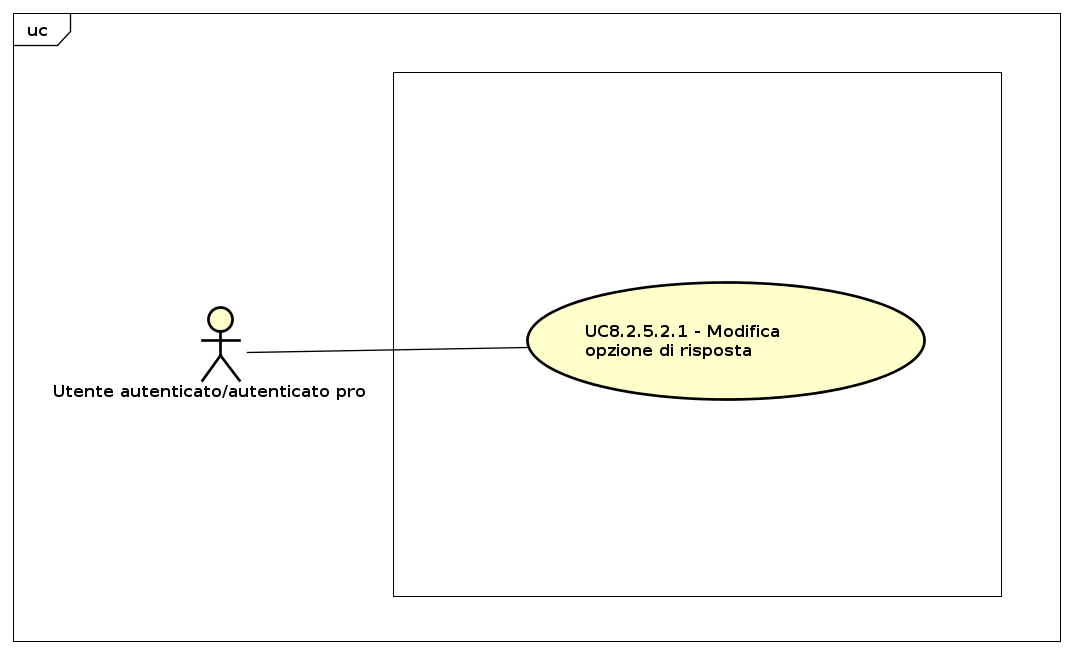
\includegraphics[scale=0.45,keepaspectratio]{UML/UC8_2_5_2.png}
		\caption{UC8.2.5.2: Selezione modalità di risposta a scelta multipla}
	\end{figure}
	\FloatBarrier	
	\begin{itemize}
		\item
			\textbf{Attori}: Utente autenticato, utente autenticato pro;
		\item
			\textbf{Scopo e descrizione}: L'utente autenticato seleziona la modalità di risposta a scelta multipla;
		\item		
			\textbf{Precondizione}: Il sistema presenta all'utente autenticato la checkbox per selezionare la modalità di risposta a scelta multipla;
		\item
			\textbf{Scenario principale}:
				\begin{enumerate}
					\item 	
						L'utente modifica le opzioni di risposta [UC8.2.5.2.1];	
				\end{enumerate}
		\item
			\textbf{Postcondizione}: La modalità di risposta a scelta multipla è stata selezionata.
	\end{itemize}
		\subsubsection{Caso d'uso UC8.2.5.2.1: Modifica opzione di risposta}
		\begin{itemize}
		\item
			\textbf{Attori}: Utente autenticato, utente autenticato pro;
		\item
			\textbf{Scopo e descrizione}: L'utente autenticato modifica le opzioni di risposta della domanda selezionata;
		\item		
			\textbf{Precondizione}: Il sistema presenta all'utente autenticato lo spazio per modificare le opzione di risposta della domanda selezionata;
		\item		
			\textbf{Postcondizione}: L'utente autenticato ha modificato le opzioni di  risposta;
		\end{itemize}
	\subsubsection{Caso d'uso UC8.2.6: Modifica risposta corretta}
		\begin{itemize}
		\item
			\textbf{Attori}: Utente autenticato, utente autenticato pro;
		\item
			\textbf{Scopo e descrizione}: L'utente autenticato modifica la risposta corretta;
		\item		
			\textbf{Precondizione}: Il sistema predispone un strumento per modificare la risposta corretta.
		\item		
			\textbf{Postcondizione}: L'utente autenticato ha modificato la risposta corretta.
		\end{itemize}
	\subsubsection{Caso d'uso UC8.2.7: Conferma modifica}
	\begin{itemize}
		\item
			\textbf{Attori}: Utente autenticato, utente autenticato pro;
		\item
			\textbf{Scopo e descrizione}: L'utente autenticato conferma la modifica dei dati della domanda selezionata;
		\item		
			\textbf{Precondizione}: Il sistema presenta all'utente autenticato l'opzione per compiere questa operazione;
		\item
			\textbf{Postcondizione}: Il sistema ha ricevuto i dati per la modifica.
	\end{itemize}		
	\subsubsection{Caso d'uso UC8.2.8: Visualizzazione errore modifica}
	\begin{itemize}
		\item
			\textbf{Attori}: Utente autenticato, utente autenticato pro;
		\item
			\textbf{Scopo e descrizione}: L'utente visualizza un messaggio d'errore nel caso si fossero verificati uno o più scenari alternativi;
		\item		
			\textbf{Precondizione}: Il sistema ha ricevuto dei dati errati per la modifica;
		\item
			\textbf{Postcondizione}: Il sistema mostra un messaggio d'errore.
	\end{itemize}	
	
	